\documentclass{article}

\usepackage{hyperref}
\hypersetup{
	colorlinks=true,
	linkcolor=blue,
	urlcolor=cyan,}
\usepackage{booktabs}
\usepackage{textgreek}

%%%%%%%%%%%%%%%%%%%%%%%%%%%%%%%%%%%%%%%%%
% Lachaise Assignment
% Structure Specification File
% Version 1.0 (26/6/2018)
%
% This template originates from:
% http://www.LaTeXTemplates.com
%
% Authors:
% Marion Lachaise & François Févotte
% Vel (vel@LaTeXTemplates.com)
%
% License:
% CC BY-NC-SA 3.0 (http://creativecommons.org/licenses/by-nc-sa/3.0/)
% 
%%%%%%%%%%%%%%%%%%%%%%%%%%%%%%%%%%%%%%%%%

%----------------------------------------------------------------------------------------
%	PACKAGES AND OTHER DOCUMENT CONFIGURATIONS
%----------------------------------------------------------------------------------------

\usepackage{amsmath,amsfonts,stmaryrd,amssymb} % Math packages

\usepackage{enumerate} % Custom item numbers for enumerations

\usepackage[ruled]{algorithm2e} % Algorithms

\usepackage[framemethod=tikz]{mdframed} % Allows defining custom boxed/framed environments

\usepackage{listings} % File listings, with syntax highlighting
\lstset{
	basicstyle=\ttfamily, % Typeset listings in monospace font
}

%----------------------------------------------------------------------------------------
%	DOCUMENT MARGINS
%----------------------------------------------------------------------------------------

\usepackage{geometry} % Required for adjusting page dimensions and margins

\geometry{
	paper=a4paper, % Paper size, change to letterpaper for US letter size
	top=2.5cm, % Top margin
	bottom=3cm, % Bottom margin
	left=2.5cm, % Left margin
	right=2.5cm, % Right margin
	headheight=14pt, % Header height
	footskip=1.5cm, % Space from the bottom margin to the baseline of the footer
	headsep=1.2cm, % Space from the top margin to the baseline of the header
	%showframe, % Uncomment to show how the type block is set on the page
}

%----------------------------------------------------------------------------------------
%	FONTS
%----------------------------------------------------------------------------------------

\usepackage[utf8]{inputenc} % Required for inputting international characters
\usepackage[T1]{fontenc} % Output font encoding for international characters

\usepackage{XCharter} % Use the XCharter fonts

%----------------------------------------------------------------------------------------
%	COMMAND LINE ENVIRONMENT
%----------------------------------------------------------------------------------------

% Usage:
% \begin{commandline}
%	\begin{verbatim}
%		$ ls
%		
%		Applications	Desktop	...
%	\end{verbatim}
% \end{commandline}

\mdfdefinestyle{commandline}{
	leftmargin=10pt,
	rightmargin=10pt,
	innerleftmargin=15pt,
	middlelinecolor=black!50!white,
	middlelinewidth=2pt,
	frametitlerule=false,
	backgroundcolor=black!5!white,
	frametitle={Command Line},
	frametitlefont={\normalfont\sffamily\color{white}\hspace{-1em}},
	frametitlebackgroundcolor=black!50!white,
	nobreak,
}

% Define a custom environment for command-line snapshots
\newenvironment{commandline}{
	\medskip
	\begin{mdframed}[style=commandline]
}{
	\end{mdframed}
	\medskip
}

%----------------------------------------------------------------------------------------
%	FILE CONTENTS ENVIRONMENT
%----------------------------------------------------------------------------------------

% Usage:
% \begin{file}[optional filename, defaults to "File"]
%	File contents, for example, with a listings environment
% \end{file}

\mdfdefinestyle{file}{
	innertopmargin=1.6\baselineskip,
	innerbottommargin=0.8\baselineskip,
	topline=false, bottomline=false,
	leftline=false, rightline=false,
	leftmargin=2cm,
	rightmargin=2cm,
	singleextra={%
		\draw[fill=black!10!white](P)++(0,-1.2em)rectangle(P-|O);
		\node[anchor=north west]
		at(P-|O){\ttfamily\mdfilename};
		%
		\def\l{3em}
		\draw(O-|P)++(-\l,0)--++(\l,\l)--(P)--(P-|O)--(O)--cycle;
		\draw(O-|P)++(-\l,0)--++(0,\l)--++(\l,0);
	},
	nobreak,
}

% Define a custom environment for file contents
\newenvironment{file}[1][File]{ % Set the default filename to "File"
	\medskip
	\newcommand{\mdfilename}{#1}
	\begin{mdframed}[style=file]
}{
	\end{mdframed}
	\medskip
}

%----------------------------------------------------------------------------------------
%	NUMBERED QUESTIONS ENVIRONMENT
%----------------------------------------------------------------------------------------

% Usage:
% \begin{question}[optional title]
%	Question contents
% \end{question}

\mdfdefinestyle{question}{
	innertopmargin=1.2\baselineskip,
	innerbottommargin=0.8\baselineskip,
	roundcorner=5pt,
	nobreak,
	singleextra={%
		\draw(P-|O)node[xshift=1em,anchor=west,fill=white,draw,rounded corners=5pt]{%
		Question \theQuestion\questionTitle};
	},
}

\newcounter{Question} % Stores the current question number that gets iterated with each new question

% Define a custom environment for numbered questions
\newenvironment{question}[1][\unskip]{
	\bigskip
	\stepcounter{Question}
	\newcommand{\questionTitle}{~#1}
	\begin{mdframed}[style=question]
}{
	\end{mdframed}
	\medskip
}

%----------------------------------------------------------------------------------------
%	WARNING TEXT ENVIRONMENT
%----------------------------------------------------------------------------------------

% Usage:
% \begin{warn}[optional title, defaults to "Warning:"]
%	Contents
% \end{warn}

\mdfdefinestyle{warning}{
	topline=false, bottomline=false,
	leftline=false, rightline=false,
	nobreak,
	singleextra={%
		\draw(P-|O)++(-0.5em,0)node(tmp1){};
		\draw(P-|O)++(0.5em,0)node(tmp2){};
		\fill[black,rotate around={45:(P-|O)}](tmp1)rectangle(tmp2);
		\node at(P-|O){\color{white}\scriptsize\bf !};
		\draw[very thick](P-|O)++(0,-1em)--(O);%--(O-|P);
	}
}

% Define a custom environment for warning text
\newenvironment{warn}[1][Warning:]{ % Set the default warning to "Warning:"
	\medskip
	\begin{mdframed}[style=warning]
		\noindent{\textbf{#1}}
}{
	\end{mdframed}
}

%----------------------------------------------------------------------------------------
%	INFORMATION ENVIRONMENT
%----------------------------------------------------------------------------------------

% Usage:
% \begin{info}[optional title, defaults to "Info:"]
% 	contents
% 	\end{info}

\mdfdefinestyle{info}{%
	topline=false, bottomline=false,
	leftline=false, rightline=false,
	nobreak,
	singleextra={%
		\fill[black](P-|O)circle[radius=0.4em];
		\node at(P-|O){\color{white}\scriptsize\bf i};
		\draw[very thick](P-|O)++(0,-0.8em)--(O);%--(O-|P);
	}
}

% Define a custom environment for information
\newenvironment{info}[1][Info:]{ % Set the default title to "Info:"
	\medskip
	\begin{mdframed}[style=info]
		\noindent{\textbf{#1}}
}{
	\end{mdframed}
}
 % Include the file specifying the document structure and custom commands

%----------------------------------------------------------------------------------------
%	ASSIGNMENT INFORMATION
%----------------------------------------------------------------------------------------

\title{Week 3: Electromyography (EMG) II}
\author{BIOE 320 Systems Physiology Laboratory} 
\date{}
%----------------------------------------------------------------------------------------

\begin{document}
\large
\maketitle

\section*{Objectives}
\begin{enumerate}
	\item To measure knee reflex time under different conditions using the reflex hammer
	\item To compare and correlate magnitude of hammer strike to magnitude of response via EMG activity
\end{enumerate}

\section*{Background}
Skeletal muscle control is important for most of our daily activities, from maintaining body posture to performing activities that require more precise movements. To appropriately perform muscle activities, your central nervous system needs to know the initial position of your body and the progression of movements so that adjustments can be made as needed. This information, known as proprioceptive input, can be acquired from your brain through different receptors in your eyes, joints, vestibular apparatus, skin, and muscles themselves. There are two types of muscle receptors tasked with monitoring changes in muscle length (\textbf{muscle spindles}) or muscle tension (\textbf{Golgi tendon organs}). In this lab, we will focus on the function of muscle spindles and their importance in spinal cord reflexes.\\

Muscle spindles, which are distributed throughout the fleshy part of skeletal muscles, send information to the nervous system about length or rate of change of length of a muscle. Each muscle spindle has its own afferent nerve supply and efferent nerve supply. The former carries signals from the sensory receptor to the spinal cord, while the latter carries outgoing signals from the spinal cord to the effector organ.\\

Efferent or motor nerves can be divided into alpha motor neurons, which innervate extrafusal muscle fibers, and gamma motor neurons, which innervate intrafusal muscle fibers. Afferent or sensory nerves consist of primary endings that can detect changes in muscle length and the speed at which that change occurs, and secondary endings that detect only changes in muscle length.\\

\begin{figure}[h]
\centering
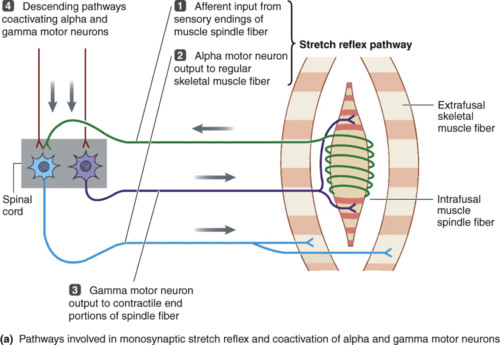
\includegraphics[width=0.8\textwidth]{../images/EMG_II_1.jpg}	
\caption{Function of muscle spindle during a monosynaptic stretch reflex.}
\label{spindle}
\end{figure}

When the muscle is passively stretched, the muscle spindles are also stretched, causing an increase in the rate of firing of the afferent nerve fibers. The afferent neuron directly synapses on the alpha motor neuron that innervates the extrafusal fibers of the same muscle, and therefore causes the muscle to contract (Fig. \ref{spindle}). This mechanism serves as a local negative feedback system that resists passive changes in muscle length so that the optimal resting length can be maintained.\\

Spinal cord reflexes represent the most basic of motor responses. These reflexes are carried out entirely within the spinal cord and are modified by inputs from higher brain centers to generate complex movements. The myotatic, or muscle stretch reflex, is an example of a spinal reflex. When the tendon is hit, the muscle and associated spindle are stretched, causing an increase in the firing rate (action potential spike frequency) of the sensory afferent neuron. This signal is relayed through the spinal cord back to the alpha motor neuron that causes the outlying muscle to contract (reflex response). A monosynaptic stretch reflex depends on three factors:

\begin{enumerate}
	\item \textbf{Reflex arc length}: distance that the signal travels from the muscle spindle to the spinal cord region where it synapses with the motor nerve and back (i.e. sensory nerve plus motor nerve path)
	\item \textbf{Nerve conduction velocity}
	\item \textbf{Synaptic transmission time}
\end{enumerate}

The \textbf{knee jerk reflex} is a spinal reflex activated by tapping the patellar tendon below the kneecap. This tendon then stretches the muscle spindles, generating sensory impulse to the spinal cord. Alpha motor neurons in the spinal cord cause a brief, rapid contraction of the quadriceps femoris, which causes the leg to extend.\\

\begin{figure}[h]
\centering
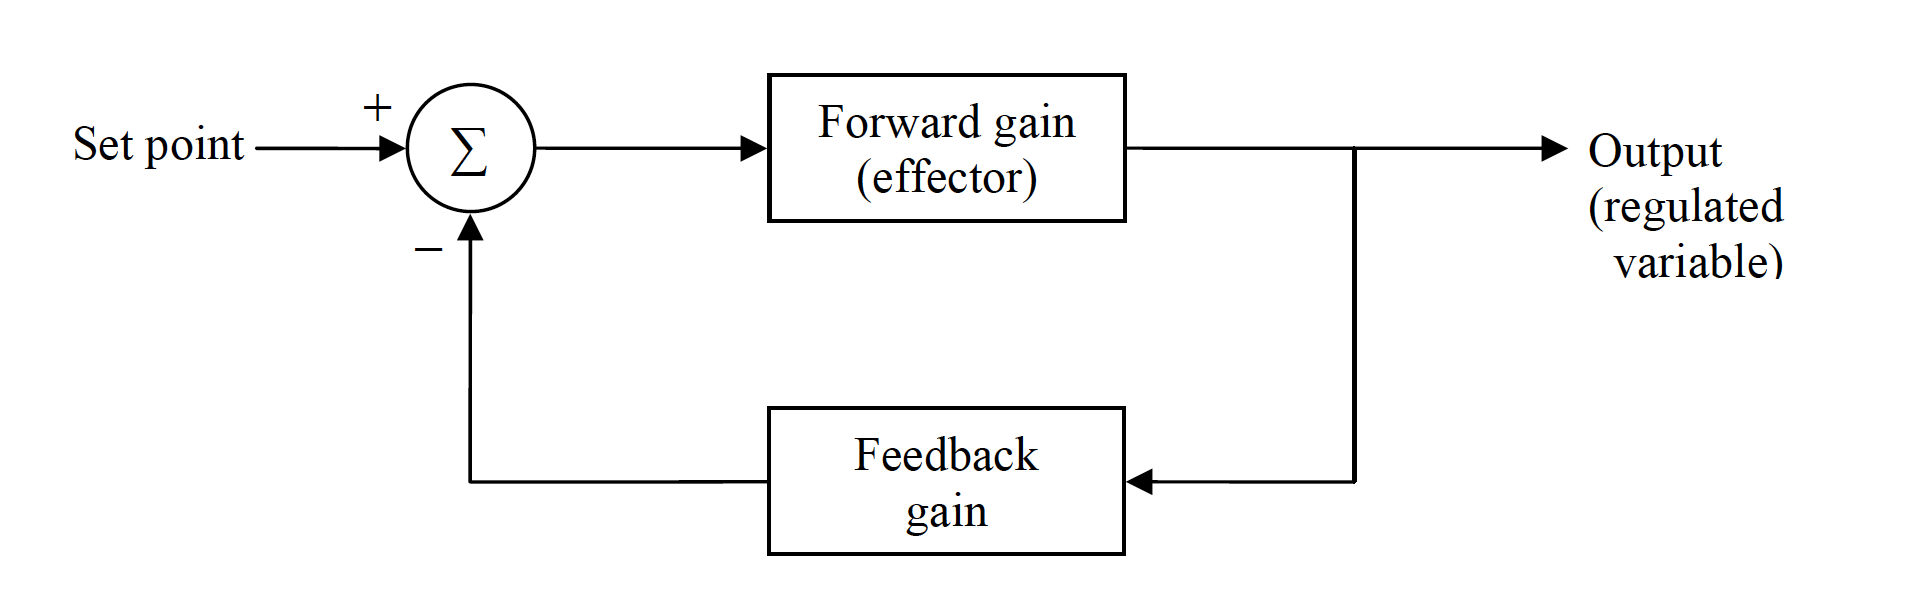
\includegraphics[width=0.9\textwidth]{../images/EMG_II_2.png}	
\caption{Function of muscle spindle during a monosynaptic stretch reflex.}
\label{feedback}
\end{figure}

This entire system can be generalized as a control system in which a regulated variable (e.g. the spike frequency of the stretch receptor) is continuously adjusted by negative feedback. Fig. \ref{feedback} shows a generalized diagram of a negative feedback control system. The set point is the desired value of the regulated variable. The forward and feedback gain represent places where the signal is multiplied by some value. The output is measured by a detector and fed back to an integrating center (the summation sign in the diagram), which takes the difference between the set point and feedback. This difference is used to control the effector responsible for the output variable. We can use this type of generalization to explore properties of the stretch reflex and how it changes.\\

\begin{enumerate}
	\item Write the physiological analog of the spinal reflex arc to each component of the negative feedback system diagram:
	\begin{enumerate}
		\item Set point:
		\item Forward gain (effector):
		\item Output (regulated variable):
		\item Feedback gain:
	\end{enumerate}
	\item What happens to the regulated output variable if it is higher than the set point? What if it is lower?
\end{enumerate}

\section*{Experimental Methods}
\subsection*{Setting Up the Software}
\begin{enumerate}
	\item Open BIOPAC student lab lessons software and select \textit{L20} (see Fig. \ref{lesson}).
	
		\begin{figure}[h]
		\centering
		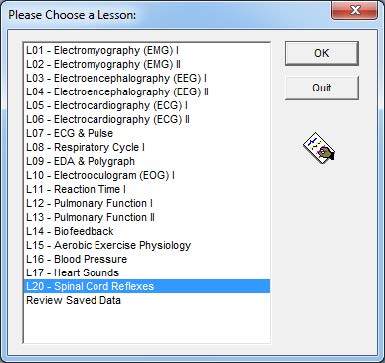
\includegraphics[width=0.6\textwidth]{../images/EMG_II_3.jpg}	
		\caption{Select lesson L20 - Spinal Cord Reflexes}
		\label{lesson}
		\end{figure}
	\item Plug the output line from the reflex hammer into channel 1 of the MP3X unit. The signal from the reflex hammer record the impact of the hammer with a surface.
	\item Plug the electrode lead set (SS2L) into channel 2. The signal from the electrodes records the EMG of the muscle activity.
\end{enumerate}

\subsection*{Calibration}
\begin{enumerate}
	\item Place two electrodes on the quadriceps muscle on the front of the thigh, approximately 10 cm apart (Fig. \ref{knee}). Connect the leads as described below:
		\begin{itemize}
			\item Red (+): closest to knee
			\item White (-): middle of calf
			\item Black (ground): inside of ankle
		\end{itemize}
		
		\begin{figure}[h]
		\centering
		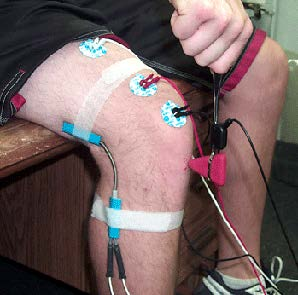
\includegraphics[width=0.5\textwidth]{../images/EMG_II_7.jpg}	
		\caption{Electrode positioning for knee jerk reflex}
		\label{knee}
		\end{figure}

	\item Click the \textit{Calibrate} button after reading through the prompts.
	\item Make sure the subject is relaxed and the hammer is placed on a flat surface. When the subject is ready, click \textit{OK} to start the calibration recordings.
	\item During the calibration procedure, start with a relaxed muscle and the hammer on a flat surface, then strike the hammer \textbf{lightly} in the table 2-3 times and flex your muscle of interest 2-3 times.
	\item The calibration procedure will stop automatically after 12 seconds. If the data resembles the plot on screen, proceed to the next section. Otherwise, recheck connections and click \textit{Redo Calibration}.
\end{enumerate}

\subsection*{Regular Procedure}
\begin{enumerate}	
	\item Have the subject sit with their legs hanging freely over the edge of the chair.
	\item Select \textit{Record} when you are ready to start recording.
	\item Strike the patellar ligament on the knee and observe the resulting reflex contraction.
	\item Continue recording and repeat the strike on the patellar ligament 15-20 times, as necessary, to get consistent data.
	\item Click on the \textit{Suspend} button to pause or stop recording.
	\item Determine the reaction times for each strike and record them on your handout. Additionally, determine the magnitude of the hammer strike and the EMG pulse for each strike. For all three measurements, calculate the mean and standard deviation.
	\item Is there a relationship between hammer strike force and reaction time? Explain.
	\item Is there are relationship between hammer strike force and the magnitude of the muscle response? Explain.
	\item Measure the length of this reflex arc, realizing that it involves the L2, L3, and L4 segments of the spinal cord. Calculate an estimate of the nerve conduction velocity. Do you expect this to be an overestimate or an underestimate? Why? \textbf{Record the conduction velocity as you will need this information for your post-lab assignment}.
	\item Do not remove the electrodes. After checking your results (and before you exit this screen and begin data analysis), continue to the following section.
\end{enumerate}

\subsection*{Jendrassik Maneuver}
\begin{enumerate}
	\item Maintain the electrodes and leads as described in the previous section.
	\item Have the subject remain seated with their legs hanging freely over the edge of the chair.
	\item Have the subject perform the Jendrassik Maneuver. To perform this maneuver, the subject must grip both hands together across their chest and attempt to pull them apart with maximum force while the knee jerk reflex is obtained (Fig. \ref{jendrassik}).
	
		\begin{figure}[h]
		\centering
		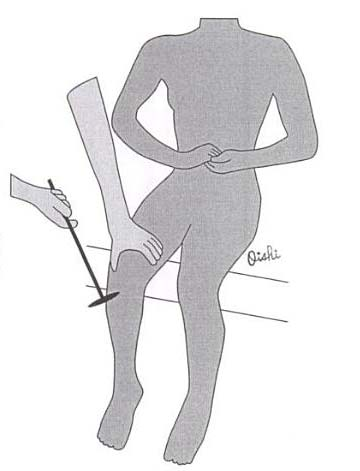
\includegraphics[width=0.4\textwidth]{../images/EMG_II_8.jpg}	
		\caption{Jendrassik maneuver}
		\label{jendrassik}
		\end{figure}

	\item Conduct the procedure given in the previous section to collect the necessary data.
	\item When you are done, select \textit{Analyze current data file.}
	\item Determine the reaction times for each strike and record them on your handout. Additionally, determine the magnitude of the hammer strike and the EMG pulse for each strike. For all three measurements, calculate the mean and standard deviation.
	\item How do the reaction times during the Jendrassik maneuver compare to the regular procedure? Explain the change or lack of change.
	\item How do the muscle response magnitudes during the Jendrassik maneuver compare to the regular procedure? Recall the negative feedback diagram (Fig. \ref{feedback}). Which variable do you think has changed?
	\item One feature of negative feedback systems with high gain is \textit{ringing}, the presence of transient oscillations in the regulated variable before it settles to a steady-state value. Did you observe ringing in any of your experiments? If so, in what test(s)? Briefly describe how this occurs in terms of the feedback diagram. Why does high gain make ringing more likely?
\end{enumerate}
\end{document}
